\newpage
\section{Comunicación en la empresa.}

La comunicación es un proceso mediante el cual intercambiamos e	
interpretamos mensajes significativos	en	un	contexto	determinado.	La	
comunicación se caracteriza	 por ser: dinámica, irreversible, compleja	
y	por	responder	a	intenciones.
Como	hemos	visto,	en	el	proceso	comunicativo	están	presentes	el	emisor,	el	receptor,	el	mensaje,	el	código,	el	contexto,	el	canal,	el	ruido	y	la	
redundancia.	Así	pues,	en	el	proceso	intervienen	 todos	los	elementos	
nombrados	y	se	pueden	distinguir	las	cuatro	fases	siguientes:

\begin{enumerate}
    \item \textbf{Fase de codificación y emisión.}	 El	emisor	siente	la	necesidad	de	
    transmitir	una	información.	Para	ello,	construye	un	mensaje	según	un	
    código	(comprensible	tanto	para	el	emisor	como	para	el	receptor)	y	
    se	lo	envía	al	receptor.

    \item \textbf{Fase de transmisión.} El	mensaje	codificado	es	transportado	a	través	del	canal	elegido,	desde	el	emisor	hacia	receptor.
    \item \textbf{Fase de recepción y descodificación.}	 El	receptor	capta	el	mensaje	
    y	lo	descodifica,	es	decir,	lo	interpreta	y	lo	comprende,	o	cree	comprenderlo.
    \item \textbf{Fase de retroalimentación.} El receptor completa el proceso de
    comunicación	 al	 transmitir	 una	 respuesta	 al	 emisor,	 es	 decir,	 lo	retroalimenta.
\end{enumerate}

\subsection{Comunicación Interna de la empresa}
La comunicación interna puede definirse como  la forma en que una empresa interactúa
con su gente y cómo estos interactúan con ella. Aquella que va dirigida al cliente
interno, el empleado. Aparece debido a las nuevas necesidades de las compañías,
en las que el empresario busca motivar a su equipo y retener a los mejores en un
entorno empresarial cambiante.  

La comunicación interna integra todos aquellos procesos involucrados en la
transmisión y recepción de información entre todos los miembros de una organización.

\subsubsection{Importancia}
Es un factor básico y repercute enormemente en los diferentes procesos de negocio de una empresa, una mejor comunicación interna mayor es el ámbito de rendimiento.

La comunicación interna es responsabilidad de los departamentos de Recursos Humanos, marketing o relaciones públicas, pero todos los departamentos de una organización pueden contribuir a ella.

A medida que pasa el tiempo, una estrategia de comunicación interna va cumpliendo objetivos y estableciendo nuevos retos con el fin de lograr la máxima eficiencia posible.

\subsubsection{Utilidad}
El deseo de informar y de ser informados en todo aquello relacionado con la empresa.

Un sistema de comunicaciones internas que funcione bien es eficaz para motivar a los empleados a esforzarse continuamente por alcanzar el objetivo común de la organización.

La comunicación interna define como la empresa se comunica y establece el camino bidireccional de la información. 

\subsubsection{Ventajas}
Son todo ventajas lo que ofrece la comunicación interna, mejorando abiertamente la gestión de una empresa:

\begin{enumerate}
    \item \textbf{Promueve y mantiene la información}
    La primera ventaja es obvia, mantiene al personal informado. Los empleados desean información sobre la empresa para la que trabajan, los proyectos en los que están trabajando y los objetivos generales de ambos.
    Aquellas empresas  con una comunicación ineficaz y oscura, pierden rendimiento y el compromiso de los empleados.
    
    \item \textbf{Crea y desarrolla la cultura empresarial}
    En cierto sentido, la función principal de las comunicaciones internas es ayudar a que la cultura de su empresa sea transparente y cercana.
    Mostrar las ideas y los valores de una empresa de un modo transparente ayuda a crear la cultura de empresa. La cultura empresarial se conforma por ambas partes, el lado de la empresa necesita la comunicación interna para mostrar todo su mensaje.
    
    \item \textbf{Crea compromiso}
    La información hace que el empleado sepa de la empresa  y pueda expresar sus opiniones. Esto lo hace sentir parte de  todo y mostrar una mayor empatía y compromiso con la empresa.
    Este compromiso deriva en lealtad y en una mayor capacidad de retención del talento.
    
    \item \textbf{Mejor ambiente de trabajo}
    Un entorno de trabajo saludable debe ser siempre un objetivo principal de una empresa. Un sistema de comunicaciones internas eficaz fomenta un entorno de trabajo abierto, comunicativo y transparente, generando una ventaja competitiva de gran valor.
\end{enumerate}

\subsubsection{Tipos de comunicación interna}
Según su contexto, la comunicación en el ámbito
laboral puede ser:

\begin{itemize}
    \item Según su \textbf{estructura}: Formal o informal
    \item Según el \textbf{código de transmisión}: oral y escrita; visual y audiovisual.
    \item Según el \textbf{ámbito:} externa e interna.
    \item Según la \textbf{dirección:} vertical y horizontal.
    \item Según el \textbf{alcance:} individual y colectiva.
    \item Según el \textbf{tema y posibilidad de acceso} a ella: Confidencial y no confidencial.
    \item 
\end{itemize}

Como hemos visto la combinación interna puede ser
tanto vertical (ascendente o descendente)

\begin{figure}[ht]
    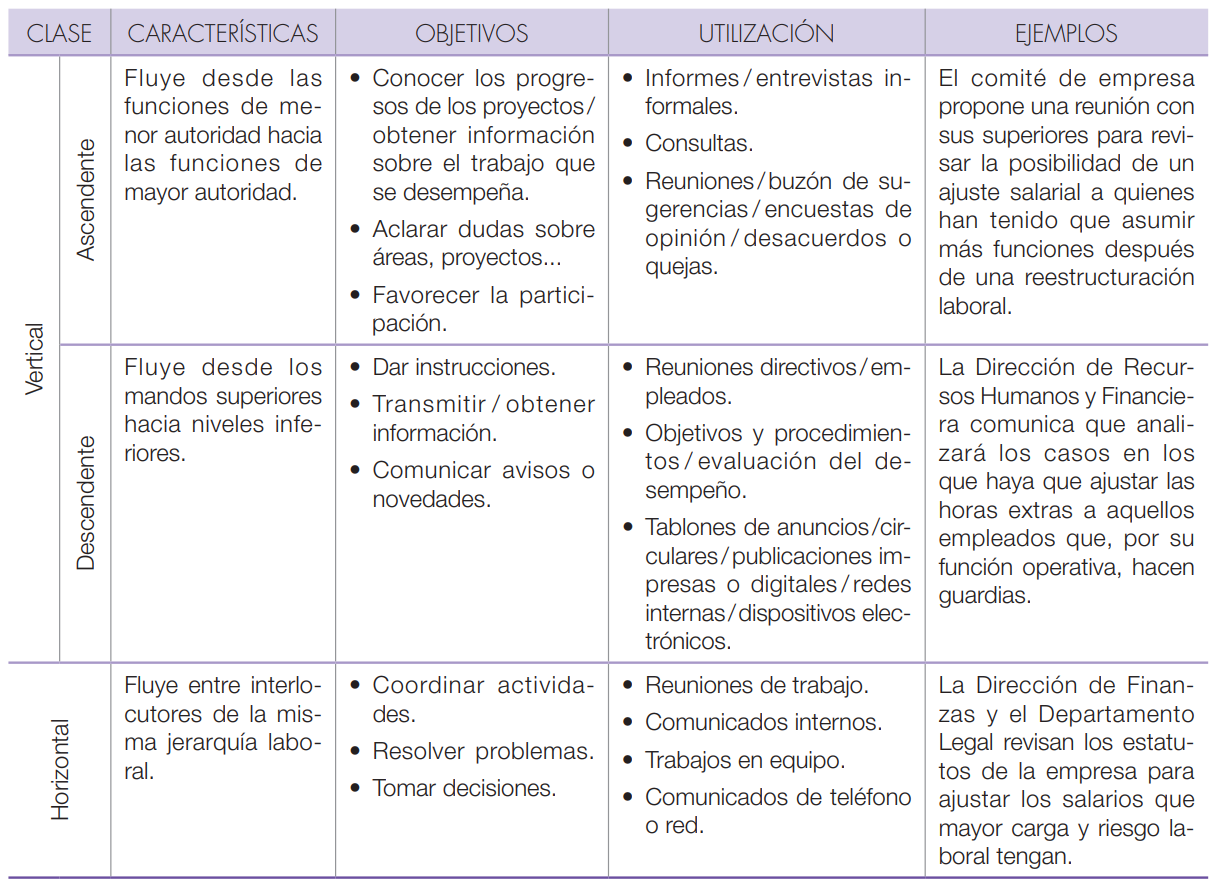
\includegraphics[scale=0.46]{sections/img/table1.png}
\end{figure}

\textbf{Comunicación según el código según el código
de transmisión empleado}

Dentro de la modalidad de comunicación empresarial, 
además de la comunicación en cuanto al ámbito
y la dirección de la información, se encuentra la
modalidad que atiende al código de transmisión
empleado, es decir, el lenguaje oral y escrito.

Teniendo en cuenta que el lenguaje humano se divide
en dos tipos, el no verbal y el verbal, el lenguaje
no verbal utiliza para expresarse signos diferentes
a las palabras, mientras que el lenguaje verbal emplea
la palabra como único medio de comunicación.

\begin{figure*}[ht]
    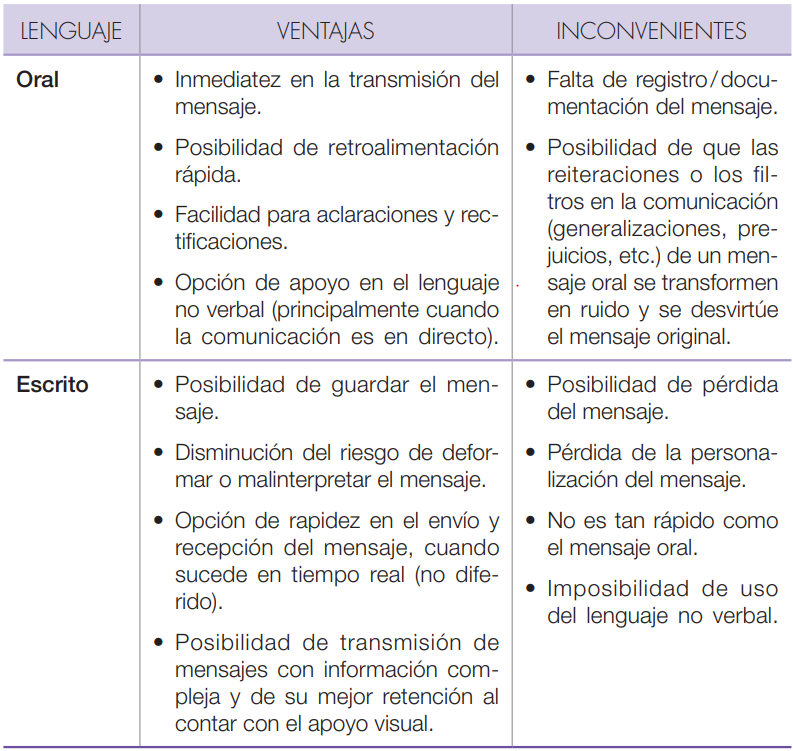
\includegraphics[scale=0.46]{sections/img/table2.png}
\end{figure*}

\subsubsection{Herramientas para desarrollar una óptima comunicación}
\begin{enumerate}
    \item \textbf{Intranet} En la época de las nuevas tecnologías y el Big Data una buena intranet ayuda a establecer contenido categorizado y facilita la búsqueda de importante y valiosa información.
    \item \textbf{Newsletter} Indispensables en la rutina de las empresas. Son ideales para enviar a tus empleados noticias interesantes sobre el sector para que se mantengan al día, eventos a los que asiste la empresa, valores o conceptos que quieres transmitir, testimonios o novedades en la empresa.
    \item \textbf{Redes sociales corporativas.} Esta herramienta ayuda a los empleados a interactuar y colaborar provocando un acercamiento entre ellos. Además de permitirles de forma más rápida y eficaz la comunicación, con la posibilidad de abrir grupos de conversación por equipos.
    \item \textbf{Buzón de sugerencias. } Esta nos ayuda a recoger las ideas, feedback u opiniones de los empleados, sabiendo cosas que pueden ser de gran ayuda para la empresa. Puede ser en formato físico o virtual. La opinión del empleado es vital para la evolución y el desarrollo de la empresa.
    \item \textbf{Reuniones. } Es una de las herramientas de comunicación más utilizada por los empresarios. Sirve para que los altos cargos interactúen con el personal, y así acercarse al equipo. Pudiendo informar, capacitar, motivar o coordinar nuevos objetivos. La previa planificación de estas y la buena decisión del lugar de su realización son puntos a favor.
\end{enumerate}

\subsubsection{Cómo elaborar un plan de comunicación interna}
Una óptima y profesional comunicación interna se sustenta bajo una estrategia o plan de comunicación
interna. ¿Por dónde empezar?.

\begin{enumerate}
    \item \textbf{¿Qué información se quiere compartir?}
    Toda estrategia de comunicación interna debe cubrir los tipos de información
    que se quieren compartir con los empleados: Objetivos, reconocimientos, logros, información sobre cambios, etc.

    \item \textbf{Directrices sobre transparencia}
    En toda comunicación se va a tener información y datos para compartir y otros que no puede serlo.
    Es muy importante, tener una idea clara de lo que se quiere compartir y lo que se desea mantener en privado o compartir más adelante.
    Independientemente del nivel de transparencia que adopte como parte del plan de comunicación interna, es básico ser siempre auténtico y directo a comunicar con los empleados
    
    \item \textbf{Establecer un horario de comunicaciones}
    Las comunicaciones cuanto más organizadas, mayor solidez y estabilidad darán a las partes interesadas.
    Este hecho lo marcará de forma directa el tipo de fuente o vía de comunicación a utilizar.
    
    \item \textbf{Canales de comunicación}
    Cuanto más rico sea el catálogo de canales de comunicación mejor se llegará los destinatarios. Así pues podemos encontrar: mensajería interna de la intranet de la empresa, publicaciones en redes sociales, aplicaciones móviles, video y correo electrónico.
    El tipo de canal a utilizar, está vinculado directamente al tipo de nicho demográfico de la empresa, la gente joven está más abierta a opciones innovadoras que los empleados de mayor edad.
    Además de todo esto, se deben asignar los responsables de la creación del plan de comunicación interna, los cuales deben ser capaces de  mantener los objetivos y fijar nuevos retos en la comunicación de la empresa.
    La comunicación interna es un proceso  en continua evolución que a medio y largo plazo ofrece muchas ventajas para ambas partes interesadas y participes en la propia comunicación.
\end{enumerate}

\subsection{La comunicación externa en la empresa}
Las organizaciones intercambian información de manera constante con su
entorno exterior. ESe entorno, dependiendo del sector y la actividad
a la que se dedique la empresa, está formado por clientes, proveedores,
competencia, intermediarios, medios de comunicación y públicos en general.

Para transmitir la información sobre la empresa al exterior, las 
organizaciones suelen emplear una serie de canales de comunicación formales
entre los que se encuentran las áreas de \textit{publicidad  y relaciones públicas,
las de marketing, prensa, etc.} Además, utilizan otros canales de comunicación informal,
que van surgiendo conforme van cambiando las necesidades de comunicación.

Dentro de los canales de comunicación mencionados, los departamentos de publicidad
y relaciones públicas son los encargados de informar al público sobre las actividades,
los productos y los servicios que ofrecen la empresa.

Tanto la publicidad como las relaciones públicas permiten dar a conocer la imagen de la empresa.

